% Provenance (never printed): see sources/outline_sources.md (Year 3:
% dislocation and diffusion creep; flow laws; deformation maps; shear zones and
% kinematic indicators). Brief: sources/book5/BRIEFS.md, ch. 7. Curves from
% figdata/bachelor-3/flow_laws.py. Exercise and problem values in the Book 5
% scratch calculator calc/ch07.py.
\chapter{Mécanismes de déformation et zones de cisaillement}\label{ch:b3:deformation-mechanisms}

En surface, le granite d'une montagne se fracture le long de failles. Vingt
kilomètres plus bas, ce même granite coule comme du caramel mou dans une \omterm{def:b3:deformation-mechanisms:shear-zone}{zone de
cisaillement} large de quelques centaines de mètres, ses feldspaths arrondis en «~yeux~» et son quartz
étiré en rubans. Un cristal peut s'écouler sans se rompre, car il n'est jamais parfait~:
il se déplace grâce à ses défauts, une rangée d'atomes à la fois, ou par des atomes qui diffusent
d'une face d'un grain à l'autre. Ce chapitre suit ces mécanismes depuis le
réseau cristallin jusqu'aux lois qu'utilise la géodynamique, aux cartes qui indiquent quel
mécanisme l'emporte, et jusqu'aux \omterm{def:b3:deformation-mechanisms:shear-zone}{zones de cisaillement} où la roche enregistre son mouvement.

\begin{recall}
Les défauts ponctuels, la loi d'Arrhénius et l'énergie d'activation sont traités dans les
volumes de chimie universitaires~; le coefficient de diffusion dans les
volumes de physique. Contrainte et déformation, l'ellipse de déformation, le cisaillement simple et son ellipse
($S_{1,2} = \sqrt{1 + \gamma^2/4} \pm \gamma/2$, grand axe à $\theta'$ de la
direction de cisaillement, avec $\tan2\theta' = 2/\gamma$), fluage en loi de puissance avec ses
constantes pour le quartzite humide et l'olivine sèche, l'enveloppe de résistance et la
transition cassant--ductile figurent dans le volume de première année, dans son chapitre sur
contrainte, déformation et rhéologie~; foliation, linéation et la description
de la mylonite dans son chapitre sur les failles, les plis et les fabriques. La
viscosité effective du manteau figure au \cref{ch:b3:mantle-convection}.
\end{recall}

\section{Défauts cristallins}

Pour cisailler un cristal parfait, toutes les liaisons traversant un plan réticulaire
devraient rompre d'un coup, ce qui demande une contrainte de l'ordre d'un dixième du
module de cisaillement, qui dans le manteau vaut environ \qty{8e10}{Pa}
(\cref{ch:b3:mantle-convection})~: des milliers de mégapascals. Les cristaux réels
cèdent sous des contraintes bien plus faibles, car ils glissent une ligne d'atomes à la fois.

\begin{definition}[Dislocation]\label{def:b3:deformation-mechanisms:dislocation}
Une \emph{dislocation}\index{dislocation (défaut cristallin)} est un défaut linéaire dans un
cristal~: la frontière, à l'intérieur du cristal, entre une partie d'un plan
réticulaire qui a glissé et une partie qui ne l'a pas. Son \emph{vecteur de Burgers}
$\mathbf b$ est le glissement qu'il transporte, égal à un pas du réseau selon une
direction du réseau. Dans une dislocation coin, $\mathbf b$ est perpendiculaire à la ligne,
qui est l'arête d'un demi-plan supplémentaire d'atomes~; dans une dislocation vis, elle
est parallèle à la ligne. Une dislocation se déplace par \emph{glissement} sur son plan de glissement,
et une dislocation coin quitte ce plan par \emph{montée}~: des atomes ou des
lacunes diffusent vers l'arête de son demi-plan ou en partent.
\end{definition}

\begin{omfigure}
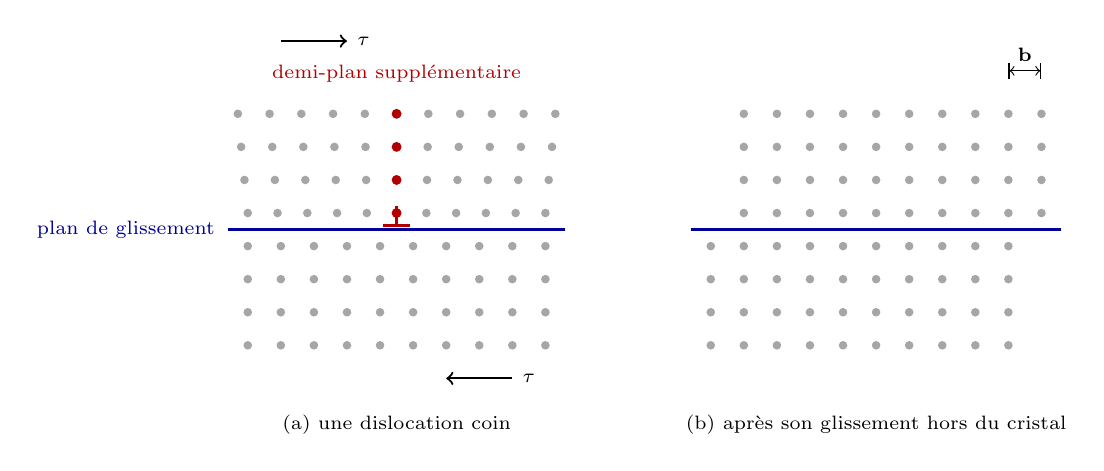
\begin{tikzpicture}[font=\scriptsize, x=0.42cm, y=0.42cm]
% (a) lower half: 10 columns; upper half: 11 columns squeezed over the same width
\foreach \j in {0,...,3} {\foreach \i in {0,...,9} {\fill[gray!70] (\i,\j) circle (0.13);}}
\foreach \j/\s in {4/0.9, 5/0.92, 6/0.94, 7/0.96} {\foreach \i in {0,...,10} {
  \pgfmathsetmacro{\x}{(\i-5)*\s + 4.5}
  \ifnum\i=5 \fill[red!70!black] (\x,\j) circle (0.15); \else \fill[gray!70] (\x,\j) circle (0.13); \fi}}
\draw[thick, blue!60!black] (-0.6,3.5) -- (9.6,3.5);
\node[anchor=east, blue!60!black] at (-0.7,3.5) {plan de glissement};
\draw[red!70!black, very thick] (4.1,3.62) -- (4.9,3.62) (4.5,3.62) -- (4.5,4.2);
\node[red!70!black] at (4.5,8.2) {demi-plan supplémentaire};
\draw[->, thick] (1.0,9.2) -- (3.0,9.2) node[right] {$\tau$};
\draw[<-, thick] (6.0,-1.0) -- (8.0,-1.0) node[right] {$\tau$};
% (b) after glide: the upper half shifted by one spacing
\begin{scope}[shift={(14,0)}]
\foreach \j in {0,...,3} {\foreach \i in {0,...,9} {\fill[gray!70] (\i,\j) circle (0.13);}}
\foreach \j in {4,...,7} {\foreach \i in {1,...,10} {\fill[gray!70] (\i,\j) circle (0.13);}}
\draw[thick, blue!60!black] (-0.6,3.5) -- (10.6,3.5);
\draw[|<->|] (9,8.3) -- (10,8.3) node[midway, above] {$\mathbf b$};
\end{scope}
\node[anchor=north] at (4.5,-1.8) {(a) une dislocation coin};
\node[anchor=north] at (19,-1.8) {(b) après son glissement hors du cristal};
\end{tikzpicture}

\par\smallskip{\small (a) Une \omterm{def:b3:deformation-mechanisms:dislocation}{dislocation} coin~: un demi-plan supplémentaire d'atomes (en rouge)
se termine sur le plan de glissement, déformant le réseau autour de son arête (le symbole
$\perp$). Sous la contrainte de cisaillement $\tau$, elle glisse le long du plan de
glissement en rompant et en reformant une rangée de liaisons à la fois. (b) Lorsqu'elle a traversé le
cristal, la moitié supérieure a glissé d'un vecteur de Burgers $\mathbf b$, et le
réseau est de nouveau parfait.}\label{fig:b3:deformation-mechanisms:dislocation}
\end{omfigure}

Le réseau s'oppose au glissement d'une \omterm{def:b3:deformation-mechanisms:dislocation}{dislocation} sous une faible contrainte, la
contrainte de Peierls, qui dépend de la force et de la direction des liaisons~:
c'est pourquoi certains systèmes de glissement d'un minéral sont faciles et d'autres difficiles. À mesure
que le cristal se déforme, les \omterm{def:b3:deformation-mechanisms:dislocation}{dislocations} se multiplient et s'enchevêtrent~; elles se bloquent
mutuellement, et le cristal durcit, à moins qu'elles ne puissent contourner les obstacles par montée ou s'annihiler, ce qui
demande une diffusion, donc de la chaleur.

\section{Mécanismes du fluage}

\begin{definition}[Mécanismes du fluage]\label{def:b3:deformation-mechanisms:creep}
Dans le \emph{fluage par dislocations}\index{fluage par dislocations}, les cristaux se déforment par
glissement des \omterm{def:b3:deformation-mechanisms:dislocation}{dislocations}, la montée les libérant des obstacles. Dans le
\emph{fluage par diffusion}\index{fluage par diffusion}, ils changent de forme par la diffusion
d'atomes, à travers le réseau (fluage de Nabarro--Herring) ou le long des
joints de grains (fluage de Coble), depuis les faces soumises à la plus forte contrainte normale
vers celles soumises à la plus faible. Dans le \emph{glissement aux joints de grains}\index{glissement aux joints de grains}
où les grains glissent les uns par rapport aux autres le long de leurs joints, les vides étant
comblés par diffusion ou par fluage par \omterm{def:b3:deformation-mechanisms:dislocation}{dislocations}. Dans la \emph{dissolution sous
pression}\index{dissolution sous pression}, la matière se dissout dans un film de fluide sur les
faces soumises à une forte contrainte et se dépose là où la contrainte est faible, ou bien
elle est emportée au loin.
\end{definition}

\begin{proposition}[Dépendance à la taille de grain du fluage par diffusion]\label{prop:b3:deformation-mechanisms:grain-size}
À faible contrainte $\sigma$, une roche de taille de grain $d$ flue par diffusion à la vitesse
\[
  \dot\varepsilon \approx B_L\frac{D_L\Omega}{k_BT}\frac{\sigma}{d^2}
  \quad\text{(à travers le réseau)},\qquad
  \dot\varepsilon \approx B_B\frac{\delta D_B\Omega}{k_BT}\frac{\sigma}{d^3}
  \quad\text{(le long des joints)},
\]
où $D_L$ et $D_B$ sont les coefficients de diffusion dans le réseau et dans les
joints, $\delta$ la largeur d'un joint, $\Omega$ le volume d'un atome,
$k_B$ la constante de Boltzmann et $B_L$, $B_B$ des nombres de l'ordre de dix qui dépendent de
la forme des grains.
\end{proposition}

\begin{proof}
Une contrainte normale $\sigma$ sur une face modifie de $\sigma\Omega$ le travail nécessaire
pour y former une lacune, de sorte que la concentration $C$ de lacunes diffère entre
les faces en traction et celles en compression, d'une quantité $\Delta C \approx C\sigma\Omega/
(k_BT)$ lorsque $\sigma\Omega \ll k_BT$. Sur une distance de l'ordre de $d$, le
flux diffusif de lacunes, donc d'atomes dans le sens opposé, est de l'ordre de $D\Delta
C/d$ par unité d'aire. À travers le réseau, le flux traverse une aire de l'ordre de
$d^2$, le long des joints, une aire de l'ordre de $\delta d$. Le volume déplacé par
unité de temps, divisé par le volume du grain $d^3$, est la vitesse de déformation~: de l'ordre de
$(D_L\sigma\Omega/k_BT)\,d^2/(d\cdot d^3) = D_L\sigma\Omega/(k_BTd^2)$ à travers le
réseau, et $(D_B\sigma\Omega/k_BT)\,\delta d/(d\cdot d^3) = \delta D_B
\sigma\Omega/(k_BTd^3)$ le long des joints. Le produit $C\,D$ est le
coefficient d'autodiffusion, noté $D$ dans l'énoncé.
\end{proof}

Le \omterm{def:b3:deformation-mechanisms:creep}{fluage par diffusion} est linéaire en la contrainte, un véritable écoulement visqueux, et il est
rapide dans les roches à grains fins~: diviser la taille de grain par deux rend le fluage de Coble huit fois plus rapide
(figure ci-dessous). Le \omterm{def:b3:deformation-mechanisms:creep}{fluage par dislocations} ne dépend pas de la taille de grain, mais croît
avec une forte puissance de la contrainte.

\begin{omfigure}
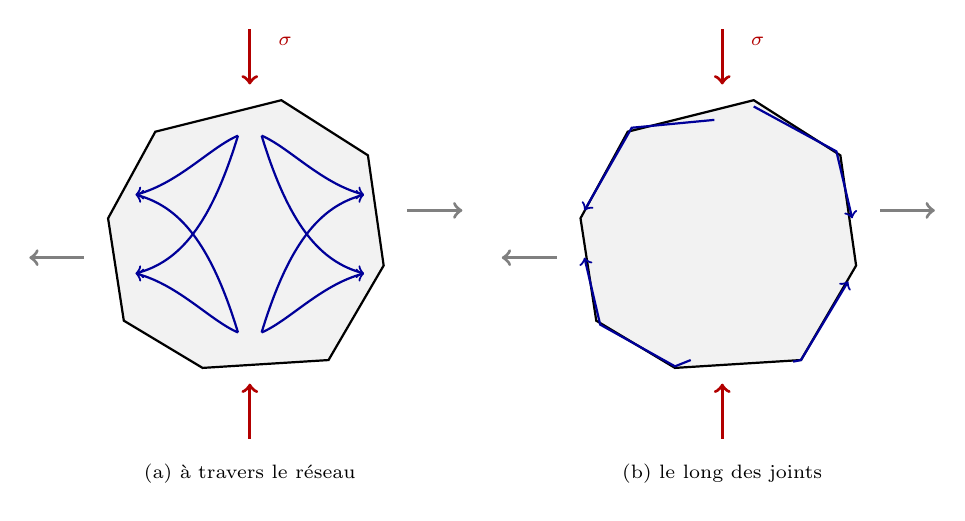
\begin{tikzpicture}[font=\scriptsize, x=1cm, y=1cm]
\foreach \cx/\lab in {0/{(a) à travers le réseau}, 6/{(b) le long des joints}} {
  \begin{scope}[shift={(\cx,0)}]
  \draw[thick, fill=gray!10] (-1.6,-1.1) -- (-0.6,-1.7) -- (1.0,-1.6) -- (1.7,-0.4) -- (1.5,1.0) -- (0.4,1.7) -- (-1.2,1.3) -- (-1.8,0.2) -- cycle;
  \draw[->, very thick, red!70!black] (0,2.6) -- (0,1.9);
  \draw[->, very thick, red!70!black] (0,-2.6) -- (0,-1.9);
  \node[red!70!black] at (0.45,2.45) {$\sigma$};
  \draw[<-, very thick, gray] (2.7,0.3) -- (2.0,0.3);
  \draw[<-, very thick, gray] (-2.8,-0.3) -- (-2.1,-0.3);
  \node[anchor=north] at (0,-2.8) {\lab};
  \end{scope}
}
\foreach \sx in {1,-1} {\foreach \y in {-0.5,0.5} {
  \draw[->, blue!60!black, thick] (0.15*\sx,1.25) .. controls (0.5*\sx,\y+0.6) and (0.9*\sx,\y+0.15) .. (1.45*\sx,\y);
  \draw[->, blue!60!black, thick] (0.15*\sx,-1.25) .. controls (0.5*\sx,\y-0.6) and (0.9*\sx,\y-0.15) .. (1.45*\sx,\y);
}}
\draw[->, blue!60!black, thick] (6.4,1.62) -- (7.45,1.05) -- (7.65,0.2);
\draw[->, blue!60!black, thick] (5.9,1.45) -- (4.85,1.35) -- (4.25,0.3);
\draw[->, blue!60!black, thick] (6.9,-1.62) -- (7.0,-1.6) -- (7.6,-0.6);
\draw[->, blue!60!black, thick] (5.6,-1.6) -- (5.4,-1.68) -- (4.45,-1.15) -- (4.25,-0.3);
\end{tikzpicture}

\par\smallskip{\small \omterm{def:b3:deformation-mechanisms:creep}{Fluage par diffusion} d'un grain raccourci selon $\sigma$. Les atomes
quittent les faces soumises à la compression la plus forte et s'ajoutent aux faces soumises
à la plus faible (en bleu), de sorte que le grain s'aplatit et s'allonge (flèches grises)~: (a)
à travers l'intérieur du grain, fluage de Nabarro--Herring~; (b) le long de ses joints,
fluage de Coble.}\label{fig:b3:deformation-mechanisms:diffusion}
\end{omfigure}

Les cristaux déformés se réparent aussi pendant qu'ils se déforment.

\begin{definition}[Restauration, sous-grain, recristallisation dynamique]\label{def:b3:deformation-mechanisms:recrystallisation}
La \emph{restauration}\index{restauration (plasticité cristalline)} est le réarrangement des
\omterm{def:b3:deformation-mechanisms:dislocation}{dislocations}, par montée et glissement dévié, en arrangements de plus basse énergie, ainsi que leur
annihilation. Des \omterm{def:b3:deformation-mechanisms:dislocation}{dislocations} disposées en parois divisent un grain en
\emph{sous-grains}\index{sous-grain}, parties du grain dont les réseaux sont inclinés
de quelques degrés les uns par rapport aux autres. \emph{Recristallisation
dynamique}\index{recristallisation dynamique} est le remplacement, pendant la
déformation, des grains écrouis par de nouveaux grains contenant moins de \omterm{def:b3:deformation-mechanisms:dislocation}{dislocations}, soit
par la rotation des sous-grains jusqu'à ce qu'ils deviennent des grains, soit par la migration
des joints de grains dans les voisins les plus déformés.
\end{definition}

\begin{definition}[Orientation cristallographique préférentielle]\label{def:b3:deformation-mechanisms:cpo}
Une roche présente une \emph{orientation cristallographique préférentielle}\index{orientation cristallographique préférentielle}
(OCP) lorsque les réseaux de ses grains ne sont pas orientés
au hasard mais se regroupent autour de directions imposées par la déformation~; le \omterm{def:b3:deformation-mechanisms:creep}{fluage
par dislocations} la produit, en faisant tourner les systèmes de glissement de chaque grain vers l'écoulement.
\end{definition}

Une roche à OCP hérite de l'anisotropie de ses cristaux~: ses vitesses sismiques, par exemple,
dépendent de la direction, ce qui permet à la sismologie de voir la fabrique
du manteau profond. Le \omterm{def:b3:deformation-mechanisms:creep}{fluage par diffusion} et le \omterm{def:b3:deformation-mechanisms:creep}{glissement aux joints de grains}, qui laissent les grains
tourner librement, n'en construisent pas.

\section{Lois de fluage}

\begin{definition}[Loi de fluage, exposant de contrainte, température homologue]\label{def:b3:deformation-mechanisms:flow-law}
Une \emph{loi de fluage}\index{loi de fluage} donne la vitesse de déformation d'une roche qui se déforme par
un seul mécanisme, en fonction de la contrainte différentielle $\sigma$, de la taille de grain
$d$, de la température $T$ et de la pression $P$~:
\[
  \dot\varepsilon = A\,\sigma^nd^{-m}\exp\Bigl(-\frac{E + PV}{RT}\Bigr),
\]
avec $A$, $n$, $m$, l'énergie d'activation $E$ et le volume d'activation $V$
mesurés en laboratoire. Le \emph{exposant de contrainte}\index{exposant de contrainte}
est $n$, l'exposant de taille de grain $m$. La \emph{température
homologue}\index{température homologue} d'un minéral est $T/T_m$, sa température absolue
divisée par sa température de fusion absolue.
\end{definition}

Dans les lois utilisées ici, le \omterm{def:b3:deformation-mechanisms:creep}{fluage par dislocations} a $n$ de 3.5 ou 4 et $m = 0$~;
le \omterm{def:b3:deformation-mechanisms:creep}{fluage par diffusion} a $n = 1$ et $m = 2$ ou 3 (voir la \cref{prop:b3:deformation-mechanisms:grain-size}).
Le fluage croît lorsque la \omterm{def:b3:deformation-mechanisms:flow-law}{température homologue} s'approche de 1. La forstérite fond à \qty{1890}{\celsius}, donc le manteau à \qty{1300}{\celsius}
se situe à $T/T_m = 0.73$~; la glace à \qty{-10}{\celsius} atteint 0.96, ce qui explique pourquoi les glaciers
s'écoulent. Les valeurs de l'olivine utilisées ici sont celles
d'une compilation de laboratoire largement employée~: olivine sèche en \omterm{def:b3:deformation-mechanisms:creep}{fluage par dislocations}, $A =
\num{1.1e5}$, $n = 3.5$, $E = \qty{530}{kJ.mol^{-1}}$, $V =
\qty{14}{cm^3.mol^{-1}}$~; en \omterm{def:b3:deformation-mechanisms:creep}{fluage par diffusion}, $A = 10^{9.2}$, $n = 1$, $m = 3$,
$E = \qty{375}{kJ.mol^{-1}}$, $V = \qty{5}{cm^3.mol^{-1}}$ (contrainte en mégapascals,
taille de grain en micromètres, temps en secondes)~; le quartzite humide est celui du
volume de première année. L'eau affaiblit l'olivine~: à une fugacité d'eau d'environ
\qty{300}{MPa}, les agrégats d'olivine fluent cinq à six fois plus vite que les
agrégats secs en \omterm{def:b3:deformation-mechanisms:creep}{fluage par dislocations}, cinq fois plus vite en \omterm{def:b3:deformation-mechanisms:creep}{fluage par diffusion}.
% ledger: bowen14:mgo-sio2, azuma17:olivine, lopez:flow-laws, codata:R, mk00:diffusion, mk00:dislocation

\begin{proposition}[Viscosité effective]\label{prop:b3:deformation-mechanisms:viscosity}
Une roche obéissant à une \omterm{def:b3:deformation-mechanisms:flow-law}{loi de fluage} $\dot\varepsilon = A'\sigma^n$ à $T$, $P$ et
$d$ donnés, a pour viscosité effective
\[
  \eta_{\mathrm{eff}} = \frac{\sigma}{2\dot\varepsilon}
  = \tfrac12A'^{-1/n}\,\dot\varepsilon^{(1-n)/n}~:
\]
pour $n > 1$, elle diminue à mesure que la roche se déforme plus vite.
\end{proposition}

\begin{proof}
Pour un fluide newtonien, $\sigma = 2\eta\dot\varepsilon$ dans un écoulement uniaxial, par
définition de la viscosité~; $\eta_{\mathrm{eff}}$ est la viscosité du fluide newtonien
qui s'écoulerait à la même vitesse sous la même contrainte. En substituant
$\sigma = (\dot\varepsilon/A')^{1/n}$, on obtient la seconde forme.
\end{proof}

Du quartzite humide à \qty{400}{\celsius}, s'écoulant à \qty{e-14}{s^{-1}}, nécessite
\qty{65}{MPa} et possède une viscosité effective de \qty{3.3e21}{Pa.s}~; à
\qty{500}{\celsius}, \qty{18}{MPa} et \qty{9e20}{Pa.s}~: une centaine de degrés
divise la résistance par plus de trois (figure ci-dessous). De l'olivine sèche à
\qty{1100}{\celsius} et \qty{1}{GPa} ne nécessite que \qty{3}{MPa}. Les enveloppes de
résistance du volume de première année sont construites précisément à partir de ces lois.

\begin{omfigure}
\begin{tikzpicture}
\begin{groupplot}[group style={group size=2 by 1, horizontal sep=1.6cm},
  omrecord, width=0.47\linewidth, height=0.47\linewidth, xmode=log,
  xmin=1, xmax=1000, ymin=-20, ymax=-6, xlabel={contrainte différentielle (MPa)},
  legend style={font=\scriptsize, at={(0.97,0.03)}, anchor=south east, legend columns=1}]
\nextgroupplot[ylabel={$\log_{10}\dot\varepsilon$ (\unit{s^{-1}})}, title={(a) quartzite humide},
  title style={font=\small}]
% computed in figdata/bachelor-3/flow_laws.py; ledger: lopez:flow-laws, azuma17:olivine
\addplot[omDef, thick] table[x=s, y=r600] {figdata/out/bachelor-3-flow_laws-quartz.dat};
\addlegendentry{\qty{600}{\celsius}}
\addplot[red!70!black, thick, densely dashed] table[x=s, y=r500] {figdata/out/bachelor-3-flow_laws-quartz.dat};
\addlegendentry{\qty{500}{\celsius}}
\addplot[black, thick, densely dotted] table[x=s, y=r400] {figdata/out/bachelor-3-flow_laws-quartz.dat};
\addlegendentry{\qty{400}{\celsius}}
\draw[gray] (axis cs:1,-14) -- (axis cs:1000,-14);
\nextgroupplot[title={(b) olivine sèche, \qty{1}{GPa}}, title style={font=\small}]
\addplot[omDef, thick] table[x=s, y=r1300] {figdata/out/bachelor-3-flow_laws-olivine.dat};
\addlegendentry{\qty{1300}{\celsius}}
\addplot[red!70!black, thick, densely dashed] table[x=s, y=r1100] {figdata/out/bachelor-3-flow_laws-olivine.dat};
\addlegendentry{\qty{1100}{\celsius}}
\addplot[black, thick, densely dotted] table[x=s, y=r900] {figdata/out/bachelor-3-flow_laws-olivine.dat};
\addlegendentry{\qty{900}{\celsius}}
\draw[gray] (axis cs:1,-14) -- (axis cs:1000,-14);
\end{groupplot}
\end{tikzpicture}

\par\smallskip{\small Lois de \omterm{def:b3:deformation-mechanisms:creep}{fluage par dislocations}~: vitesse de déformation en fonction de la contrainte à
trois températures. La pente sur ces axes est l'\omterm{def:b3:deformation-mechanisms:flow-law}{exposant de contrainte}, 4 pour
le quartzite et 3.5 pour l'olivine~; la ligne grise marque une vitesse de déformation géologique,
\qty{e-14}{s^{-1}}. L'olivine a besoin de températures d'environ \qty{600}{\celsius} plus élevées
que le quartz pour s'écouler aussi facilement.}\label{fig:b3:deformation-mechanisms:flow-laws}
\end{omfigure}

\section{Cartes des mécanismes de déformation}

Plusieurs mécanismes fonctionnent en parallèle, et le plus rapide porte la déformation.

\begin{definition}[Carte des mécanismes de déformation]\label{def:b3:deformation-mechanisms:deformation-map}
Une \emph{carte des mécanismes de déformation}\index{carte des mécanismes de déformation} d'un
minéral ou d'une roche montre, sur des axes de deux des variables contrainte, taille de grain et
température, les domaines dans lesquels chaque mécanisme est le plus rapide, avec des courbes d'isovaleur
de la vitesse de déformation totale.
\end{definition}

\begin{proposition}[Frontière entre mécanismes]\label{prop:b3:deformation-mechanisms:boundary}
À $T$ et $P$ donnés, le \omterm{def:b3:deformation-mechanisms:creep}{fluage par dislocations} ($A_1$, $n_1$, $E_1$, $V_1$, sans
dépendance à la taille de grain) et le \omterm{def:b3:deformation-mechanisms:creep}{fluage par diffusion} ($A_2$, $n_2 = 1$, $m$, $E_2$, $V_2$)
s'écoulent à la même vitesse pour la contrainte
\[
  \sigma_b = \biggl(\frac{A_2d^{-m}}{A_1}
  \exp\frac{(E_1 - E_2) + P(V_1 - V_2)}{RT}\biggr)^{1/(n_1 - 1)} ,
\]
de sorte que la frontière est une droite de pente $-m/(n_1 - 1)$ sur des axes logarithmiques
de taille de grain et de contrainte~; le \omterm{def:b3:deformation-mechanisms:creep}{fluage par dislocations} l'emporte au-dessus.
\end{proposition}

\begin{proof}
Égaler les deux \omterm{def:b3:deformation-mechanisms:flow-law}{lois de fluage} et résoudre en $\sigma$. Au-dessus de $\sigma_b$, le rapport
des deux vitesses, proportionnel à $\sigma^{n_1 - 1}$, dépasse 1.
\end{proof}

Pour l'olivine sèche à \qty{1100}{\celsius} et \qty{2}{GPa}, la frontière se situe à
\qty{5}{MPa} pour une taille de grain de \qty{1}{mm} et à \qty{79}{MPa} pour
\qty{100}{\micro m} (figure ci-dessous). Le manteau à grains fins flue par diffusion,
le manteau à gros grains par \omterm{def:b3:deformation-mechanisms:dislocation}{dislocations}~; les données de laboratoire et géophysiques suggèrent
que les deux régimes existent dans le manteau supérieur, le manteau chaud et peu profond s'écoulant par
\omterm{def:b3:deformation-mechanisms:creep}{fluage par dislocations} et le manteau plus froid ou plus profond par \omterm{def:b3:deformation-mechanisms:creep}{fluage par diffusion}, et que là où
la contrainte augmente et où les grains rétrécissent, le manteau près de la frontière s'affaiblit
et la déformation se localise.
% ledger: azuma17:olivine, karato93:transitions

\begin{omfigure}
\begin{tikzpicture}
\begin{axis}[omrecord, xmode=log, ymode=log, width=0.78\linewidth, height=0.58\linewidth,
  xmin=10, xmax=1e4, ymin=0.01, ymax=1000, xlabel={taille de grain (\unit{\micro m})},
  ylabel={contrainte différentielle (MPa)}, clip=true]
% computed in figdata/bachelor-3/flow_laws.py; ledger: azuma17:olivine
\addplot[black, very thick] table[x=d, y=s] {figdata/out/bachelor-3-flow_laws-mapbound.dat};
\foreach \c in {16,14,12,10} {
  \addplot[omDef, thick] table[x=d, y=s\c] {figdata/out/bachelor-3-flow_laws-mapcont.dat};
}
\node[font=\scriptsize, fill=white, inner sep=1pt] at (axis cs:7000,1.15) {$10^{-16}$};
\node[font=\scriptsize, fill=white, inner sep=1pt] at (axis cs:7000,4.2) {$10^{-14}$};
\node[font=\scriptsize, fill=white, inner sep=1pt] at (axis cs:7000,15.7) {$10^{-12}$};
\node[font=\scriptsize, fill=white, inner sep=1pt] at (axis cs:4200,58) {$10^{-10}\,\unit{s^{-1}}$};
\node[font=\small, anchor=north east] at (axis cs:9000,600) {fluage par dislocations};
\node[font=\small, anchor=south west] at (axis cs:1500,0.013) {fluage par diffusion};
\end{axis}
\end{tikzpicture}

\par\smallskip{\small \omterm{def:b3:deformation-mechanisms:deformation-map}{Carte des mécanismes de déformation} de l'olivine sèche à
\qty{1100}{\celsius} et \qty{2}{GPa}. La ligne épaisse sépare les domaines où le
\omterm{def:b3:deformation-mechanisms:creep}{fluage par dislocations} (au-dessus) et le \omterm{def:b3:deformation-mechanisms:creep}{fluage par diffusion} (en dessous) est le plus rapide~; les lignes fines
sont des courbes d'isovaleur de la vitesse de déformation totale, horizontales là où le \omterm{def:b3:deformation-mechanisms:creep}{fluage par dislocations}, qui
ignore la taille de grain, domine.}\label{fig:b3:deformation-mechanisms:map}
\end{omfigure}

La taille de grain que produit la \omterm{def:b3:deformation-mechanisms:recrystallisation}{recristallisation dynamique} dépend de la contrainte,
et c'est ce qui fait des grains une jauge de contrainte.

\begin{definition}[Paléopiézomètre]\label{def:b3:deformation-mechanisms:piezometer}
Un \emph{paléopiézomètre}\index{paléopiézomètre} est un élément d'une roche déformée
dont la taille ou la densité est fixée par la contrainte différentielle sous laquelle il s'est formé,
étalonné en laboratoire, à partir duquel on peut lire la contrainte
d'une déformation passée.
\end{definition}

Pour le quartz, des expériences menées à \qty{1.5}{GPa} et entre 800 et \qty{1100}{\celsius},
pour des contraintes d'écoulement comprises entre 34 et \qty{268}{MPa}, ont donné des grains recristallisés allant de 46
à \qty{3.2}{\micro m}, ajustés par
\[
  D = 10^{3.56}\,\sigma^{-1.26}\qquad(D\text{ en \unit{\micro m}},\ \sigma\text{ en MPa}),
\]
sans effet détectable de la température. Une mylonite de quartz dont les
grains recristallisés mesurant \qty{20}{\micro m} de large se sont déformés sous
une contrainte d'environ \qty{62}{MPa}.
% ledger: st03:piezometer

\section{Zones de cisaillement}

\begin{definition}[Zone de cisaillement, adoucissement par la déformation]\label{def:b3:deformation-mechanisms:shear-zone}
Une \emph{zone de cisaillement}\index{zone de cisaillement} est une zone tabulaire, comprise entre des parois
peu déformées, où la déformation est concentrée et voisine d'un cisaillement simple
parallèle à la zone. Une roche subit un \emph{adoucissement par
la déformation}\index{adoucissement par la déformation} lorsque sa résistance diminue au fur et à mesure qu'elle se déforme.
\end{definition}

L'\omterm{def:b3:deformation-mechanisms:shear-zone}{adoucissement par la déformation} est ce qui maintient une \omterm{def:b3:deformation-mechanisms:shear-zone}{zone de cisaillement} étroite~: dès qu'une bande est moins résistante
que ses parois, la déformation y reste confinée. La réduction de la taille de grain par \omterm{def:b3:deformation-mechanisms:recrystallisation}{recristallisation dynamique}, qui peut
faire basculer la roche vers le \omterm{def:b3:deformation-mechanisms:creep}{fluage par diffusion}, la croissance d'une OPC qui aligne les systèmes de glissement faciles,
l'arrivée d'eau et les réactions qui rendent
des minéraux faibles, comme les micas, adoucissent toutes la roche. Les mylonites du volume de première année en sont le produit.
Dans une \omterm{def:b3:deformation-mechanisms:shear-zone}{zone de cisaillement} simple, un marqueur qui traversait la zone à angle droit est dévié
dans celle-ci~: s'il fait, à l'intérieur de la zone, un angle
$\psi$ avec sa direction initiale, le cisaillement vaut $\gamma
= \tan\psi$, et le déplacement à travers une zone de largeur $w$ est $\gamma w$.

\begin{definition}[Indicateurs cinématiques]\label{def:b3:deformation-mechanisms:kinematic}
Un \emph{indicateur cinématique}\index{indicateur cinématique} est une structure dont l'asymétrie
enregistre le \emph{sens de cisaillement}\index{sens de cisaillement}, c'est-à-dire le sens dans
lequel une paroi d'une \omterm{def:b3:deformation-mechanisms:shear-zone}{zone de cisaillement} s'est déplacée par rapport à l'autre, lu dans le plan
qui contient la linéation d'étirement et qui est perpendiculaire à la foliation.
Une \emph{fabrique S--C}\index{fabrique S--C} est un couple de foliations~: S, la
foliation des grains aplatis, oblique à la zone et tournée vers la
direction d'étirement, et C, des bandes de cisaillement parallèles à la zone. Un
\emph{système de porphyroclaste}\index{systeme de porphyroclaste@système de porphyroclaste} est un grain résistant entouré
de queues de matériau recristallisé~: dans un porphyroclaste de type $\sigma$, les queues passent d'un
côté de la ligne médiane du clast à l'autre sans la traverser~; dans un porphyroclaste de type $\delta$,
entraînées par la rotation du clast, elles la traversent. Un
\emph{poisson de mica}\index{poisson de mica} est un grain de mica en forme de losange, incliné
par rapport au plan de cisaillement, avec de fines queues qui se décalent comme celles d'un clast de type $\sigma$.
\end{definition}

\begin{omfigure}
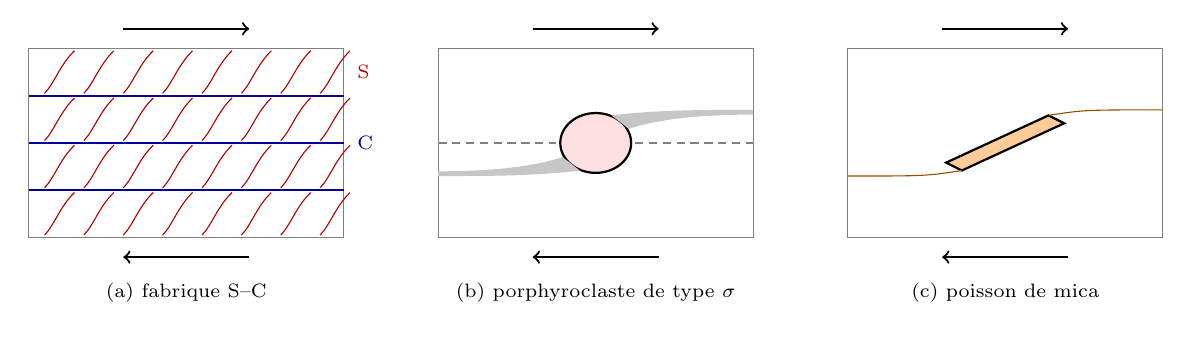
\begin{tikzpicture}[font=\scriptsize, x=1cm, y=1cm]
% (a) S-C fabric, dextral
\begin{scope}
\draw[gray] (0,0) rectangle (4,2.4);
\foreach \y in {0.6,1.2,1.8} {\draw[blue!60!black, thick] (0,\y) -- (4,\y);}
\foreach \y in {0,0.6,1.2,1.8} {\foreach \x in {0.2,0.7,...,3.8} {
  \draw[red!70!black] (\x,\y+0.03) .. controls (\x+0.12,\y+0.15) and (\x+0.2,\y+0.4) .. (\x+0.38,\y+0.57);}}
\draw[->, thick] (1.2,2.65) -- (2.8,2.65);
\draw[<-, thick] (1.2,-0.25) -- (2.8,-0.25);
\node[anchor=north] at (2,-0.45) {(a) fabrique S--C};
\node[blue!60!black, anchor=west] at (4.05,1.2) {C};
\node[red!70!black, anchor=west] at (4.05,2.1) {S};
\end{scope}
% (b) sigma clast
\begin{scope}[shift={(5.2,0)}]
\draw[gray] (0,0) rectangle (4,2.4);
\fill[red!12] (2.0,1.2) ellipse (0.45 and 0.38);
\draw[thick] (2.0,1.2) ellipse (0.45 and 0.38);
\fill[gray!45] (2.2,1.55) .. controls (2.8,1.62) and (3.3,1.62) .. (4.0,1.62) -- (4.0,1.56) .. controls (3.3,1.56) and (2.8,1.5) .. (2.42,1.38) -- cycle;
\fill[gray!45] (1.8,0.85) .. controls (1.2,0.78) and (0.7,0.78) .. (0,0.78) -- (0,0.84) .. controls (0.7,0.84) and (1.2,0.9) .. (1.58,1.02) -- cycle;
\draw[gray, densely dashed] (0,1.2) -- (1.5,1.2) (2.5,1.2) -- (4,1.2);
\draw[->, thick] (1.2,2.65) -- (2.8,2.65);
\draw[<-, thick] (1.2,-0.25) -- (2.8,-0.25);
\node[anchor=north] at (2,-0.45) {(b) porphyroclaste de type $\sigma$};
\end{scope}
% (c) mica fish
\begin{scope}[shift={(10.4,0)}]
\draw[gray] (0,0) rectangle (4,2.4);
\fill[orange!40] (1.25,0.95) -- (2.55,1.55) -- (2.75,1.45) -- (1.45,0.85) -- cycle;
\draw[thick] (1.25,0.95) -- (2.55,1.55) -- (2.75,1.45) -- (1.45,0.85) -- cycle;
\draw[orange!60!black] (2.55,1.55) .. controls (3.0,1.62) .. (4.0,1.62);
\draw[orange!60!black] (1.45,0.85) .. controls (1.0,0.78) .. (0,0.78);
\draw[->, thick] (1.2,2.65) -- (2.8,2.65);
\draw[<-, thick] (1.2,-0.25) -- (2.8,-0.25);
\node[anchor=north] at (2,-0.45) {(c) poisson de mica};
\end{scope}
\end{tikzpicture}

\par\smallskip{\small Trois \omterm{def:b3:deformation-mechanisms:kinematic}{indicateurs cinématiques} d'un même cisaillement dextre
(haut vers la droite, flèches), vus dans le plan de la linéation, perpendiculaire à la foliation.
(a) La foliation S (rouge) s'incurve dans les bandes de cisaillement C (bleu),
en s'inclinant dans la direction d'étirement. (b) Les queues d'un clast de type $\sigma$
quittent son côté supérieur vers la droite et son côté inférieur vers la gauche, en se décalant
dans le sens du cisaillement sans traverser la ligne médiane (en pointillés). (c) Un
\omterm{def:b3:deformation-mechanisms:kinematic}{poisson de mica} s'incline comme S, et ses queues se décalent comme celles d'un clast de type $\sigma$. Non
à l'échelle.}\label{fig:b3:deformation-mechanisms:kinematic}
\end{omfigure}

Pris ensemble, quelques indicateurs concordants donnent le \omterm{def:b3:deformation-mechanisms:kinematic}{sens de cisaillement}
avec confiance~; un seul peut induire en erreur, car des clasts rétro-tournés et
des plis asymétriques d'autres origines existent. La photographie de l'encadré ci-dessous
montre des porphyroclastes dans une mylonite.

\begin{inthelab}[Compresser une roche dans les conditions du manteau]
\begin{minipage}[t]{0.55\linewidth}\vspace{0pt}
Dans un appareil de déformation à milieu gazeux, un cylindre de roche ou de
poudre d'olivine compactée à chaud, long d'un ou deux centimètres, est scellé dans une fine gaine métallique et
placé avec ses pistons dans un four, lui-même logé dans une cuve d'acier remplie d'un
gaz inerte comprimé qui fixe la pression de confinement, de quelques centaines
de mégapascals. Un actionneur entraîne le piston à vitesse constante, ou sous une
charge constante, tandis qu'une cellule de charge interne mesure la contrainte exercée sur
l'échantillon lui-même, à l'abri des frottements des joints d'étanchéité. L'olivine est déformée ainsi à
des températures voisines de \qty{1200}{\celsius}~; en fin d'essai, l'échantillon est
trempé, découpé, poli, puis examiné au microscope optique et au
microscope électronique, où l'on mesure sa taille de grain, ses \omterm{def:b3:deformation-mechanisms:recrystallisation}{sous-grains} et ses \omterm{def:b3:deformation-mechanisms:dislocation}{dislocations}.
\end{minipage}\hfill
\begin{minipage}[t]{0.42\linewidth}\vspace{0pt}
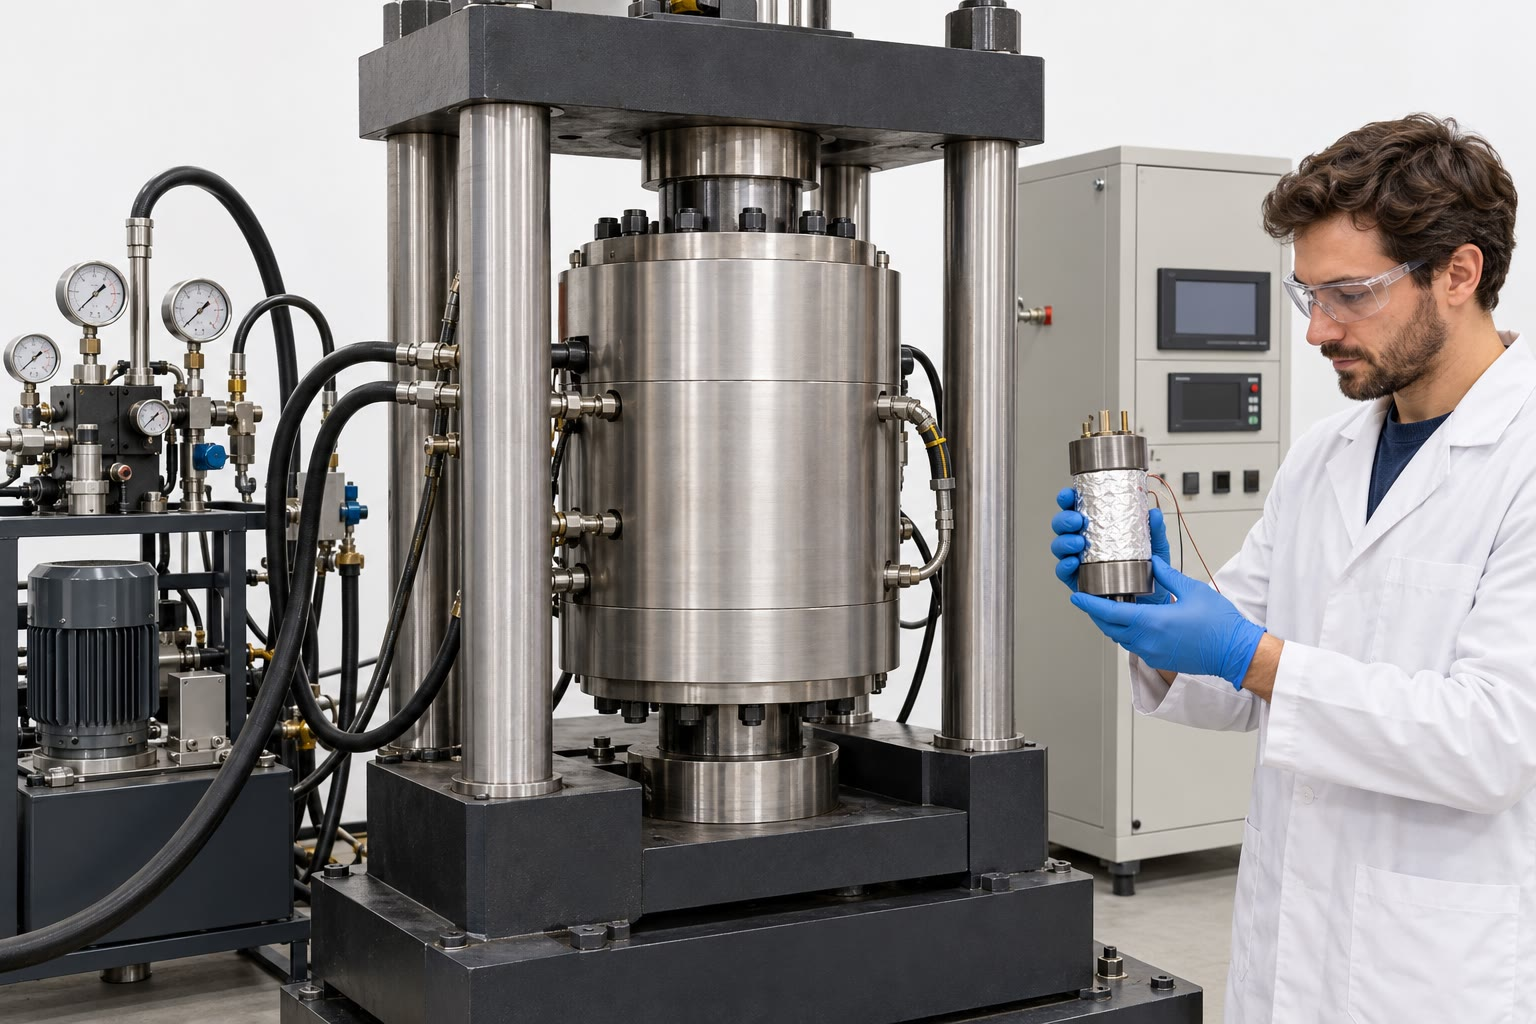
\includegraphics[width=\linewidth]{images/book5/ai/b3-deformation-press.jpg}

{\scriptsize Presse de déformation des roches avec un montage d'échantillon sous gaine
Illustration générée par IA.}

\smallskip
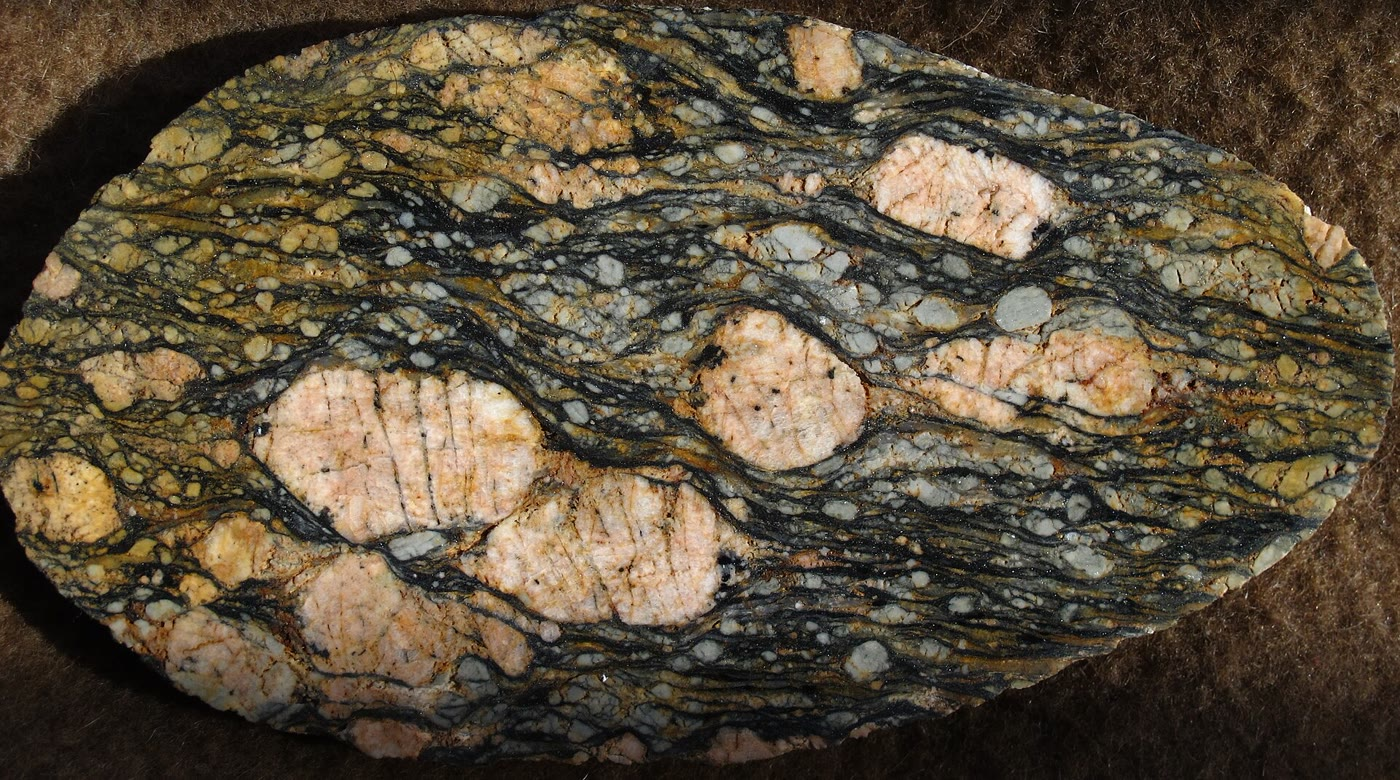
\includegraphics[width=\linewidth]{images/book5/b3-augen-mylonite.jpg}

{\scriptsize Mylonite œillée sciée provenant de Norvège~: grands porphyroclastes de feldspath
dans une fine matrice de quartz, de feldspath et de micas recristallisés. Photo
Mikenorton, CC BY-SA 4.0.}
\end{minipage}
\end{inthelab}
% ledger: mk00:diffusion, photo:b3-augen-mylonite

\section{Exercices}

\begin{exercise}[$\star$]\label{exo:b3:deformation-mechanisms:1}
La forstérite fond à \qty{1890}{\celsius} et la glace à \qty{0}{\celsius}. Calculer
la \omterm{def:b3:deformation-mechanisms:flow-law}{température homologue} de la forstérite à \qty{1300}{\celsius} et de la glace à
\qty{-10}{\celsius}. Lequel flue le plus facilement~?
\end{exercise}

\begin{exercise}[$\star$]\label{exo:b3:deformation-mechanisms:2}
Un dyke traversant une \omterm{def:b3:deformation-mechanisms:shear-zone}{zone de cisaillement} à angle droit est dévié de
\ang{70} à l'intérieur de la zone, et un autre de \ang{80}. Calculer les déformations
de cisaillement. Pourquoi les grandes déformations sont-elles difficiles à mesurer ainsi~?
\end{exercise}

\begin{exercise}[$\star$]\label{exo:b3:deformation-mechanisms:3}
Avec le \omterm{def:b3:deformation-mechanisms:piezometer}{paléopiézomètre} du quartz, quelle contrainte indique une taille de grain
recristallisée de \qty{10}{\micro m}~?
\end{exercise}

\begin{exercise}[$\star$]\label{exo:b3:deformation-mechanisms:4}
Avec la \omterm{def:b3:deformation-mechanisms:flow-law}{loi de fluage} du quartzite humide ($A = \num{1.1e-4}$, $n = 4$, $E =
\qty{223}{kJ.mol^{-1}}$, $R = \qty{8.314}{J.mol^{-1}.K^{-1}}$), calculer la
vitesse de déformation à \qty{500}{\celsius} sous \qty{20}{MPa}.
\end{exercise}

\begin{exercise}[$\star\star$]\label{exo:b3:deformation-mechanisms:5}
Calculer la viscosité effective d'un quartzite humide s'écoulant à \qty{e-14}{s^{-1}}
à \qty{400}{\celsius} (\qty{65.4}{MPa}) et à \qty{500}{\celsius}
(\qty{18.0}{MPa}). Comparer ces valeurs aux \omterm{def:b3:mantle-convection:gia}{viscosités du manteau}
étudiées au \cref{ch:b3:mantle-convection}.
\end{exercise}

\begin{exercise}[$\star\star$]\label{exo:b3:deformation-mechanisms:6}
Deux expériences à la même température donnent \qty{e-5}{s^{-1}} sous
\qty{100}{MPa} et \qty{1.6e-4}{s^{-1}} sous \qty{200}{MPa}. Calculer l'\omterm{def:b3:deformation-mechanisms:flow-law}{exposant de
contrainte} et nommer le mécanisme probable.
\end{exercise}

\begin{exercise}[$\star\star$]\label{exo:b3:deformation-mechanisms:7}
À même contrainte, un échantillon flue dix fois plus vite à \qty{1100}{K} qu'à
\qty{1000}{K}. Calculer l'énergie d'activation.
\end{exercise}

\begin{exercise}[$\star\star$]\label{exo:b3:deformation-mechanisms:8}
De quel facteur varie la vitesse de déformation en \omterm{def:b3:deformation-mechanisms:creep}{fluage par diffusion} lorsque la
taille de grain est divisée par dix, pour le fluage de Nabarro--Herring et pour le fluage de Coble~? Pourquoi le
fluage de Coble est-il le plus sensible~?
\end{exercise}

\begin{exercise}[$\star\star$]\label{exo:b3:deformation-mechanisms:9}
Pour l'olivine sèche à \qty{1100}{\celsius} et \qty{2}{GPa}, les deux \omterm{def:b3:deformation-mechanisms:flow-law}{lois de fluage} donnent
$\dot\varepsilon_{\mathrm{dis}} = \num{6.54e-17}\,\sigma^{3.5}$ et
$\dot\varepsilon_{\mathrm{dif}} = \num{3.59e-6}\,\sigma d^{-3}$ (unités du
texte). Calculer la contrainte à la frontière pour $d = \qty{1}{mm}$ et $d =
\qty{100}{\micro m}$, et la pente de la frontière.
\end{exercise}

\begin{exercise}[$\star\star\star$]\label{exo:b3:deformation-mechanisms:10}
En suivant la démonstration de la \cref{prop:b3:deformation-mechanisms:grain-size},
expliquer pourquoi le chemin par le réseau donne $d^{-2}$ et le chemin par les joints $d^{-3}$, et
montrer que la diffusion aux joints l'emporte en dessous de la taille de grain $d^* \approx
(B_B/B_L)\,\delta D_B/D_L$.
\end{exercise}

\begin{exercise}[$\star\star\star$]\label{exo:b3:deformation-mechanisms:11}
Pour une \omterm{def:b3:deformation-mechanisms:flow-law}{loi de fluage} avec $n = 3.5$, de quel facteur la viscosité effective diminue-t-elle
lorsque la vitesse de déformation est multipliée par dix~? Pourquoi cela favorise-t-il la
localisation de la déformation dans les \omterm{def:b3:deformation-mechanisms:shear-zone}{zones de cisaillement}~?
\end{exercise}

\begin{exercise}[$\star\star\star$]\label{exo:b3:deformation-mechanisms:12}
Dans l'olivine sèche de l'exercice 9, une \omterm{def:b3:deformation-mechanisms:shear-zone}{zone de cisaillement} du manteau sous \qty{10}{MPa}
se recristallise, passant de grains de \qty{3}{mm} à \qty{30}{\micro m}. Calculer la
vitesse de déformation totale avant et après, ainsi que le facteur d'adoucissement. Quel
mécanisme porte la déformation dans chaque cas~?
\end{exercise}

\section{Problème~: la zone de cisaillement de Varden}

\begin{problem}[{Problème du week-end --- la déformation, la contrainte, la vitesse de déformation et l'âge
d'une zone de cisaillement fictive}]
\label{pb:b3:deformation-mechanisms:1}
% values: calc/ch07.py; flow_laws.py; st03:piezometer, lopez:flow-laws
Sous le granite des collines de Varden, région fictive de la série, un
forage et une tranchée routière profonde (toutes deux fictives) révèlent une \omterm{def:b3:deformation-mechanisms:shear-zone}{zone de
cisaillement} ductile de \qty{400}{m} de large, formée vers \qty{15}{km} de profondeur et à \qty{450}{\celsius}.
Un dyke de dolérite qui traverse les parois à angle droit forme, à l'intérieur de la zone,
un angle de seulement \ang{6} avec les limites de la zone. Son quartz est une mylonite
de grains recristallisés de \qty{20}{\micro m} de diamètre (de 15 à
\qty{25}{\micro m}). Prendre le \omterm{def:b3:deformation-mechanisms:piezometer}{paléopiézomètre} du quartz $D = 10^{3.56}\sigma^{-1.26}$,
la \omterm{def:b3:deformation-mechanisms:flow-law}{loi de fluage} du quartzite humide ($A = \num{1.1e-4}$, $n = 4$, $E =
\qty{223}{kJ.mol^{-1}}$), $R = \qty{8.314}{J.mol^{-1}.K^{-1}}$, \qty{1}{an} $=
\qty{3.156e7}{s}$, et, en cisaillement simple, $\dot\gamma = 2\dot\varepsilon$.

\medskip\noindent\textbf{Partie I --- La déformation.}
\begin{enumerate}
  \item Calculer la déflexion $\psi$ du dyke et la déformation de cisaillement.
  \item Calculer le déplacement d'une paroi par rapport à l'autre.
  \item Calculer les étirements principaux de l'ellipse de déformation et son
        rapport d'axes.
  \item Calculer l'angle du grand axe avec la zone. Que devient la
        foliation de la zone lorsque $\gamma$ augmente~?
  \item Vu d'en haut, le dyke, suivi depuis la paroi sud, s'infléchit
        vers l'est en entrant dans la zone est--ouest, puis reprend sa
        direction vers le nord à la paroi nord. Dans quel sens la
        paroi nord s'est-elle déplacée, et la zone est-elle dextre ou senestre~?
  \item Dans quel plan faut-il prélever une lame mince pour lire les \omterm{def:b3:deformation-mechanisms:kinematic}{indicateurs
        cinématiques}, et dans quel sens doit pencher sa foliation S~?
\end{enumerate}

\medskip\noindent\textbf{Partie II --- La contrainte.}
\begin{enumerate}[resume]
  \item Calculer la contrainte indiquée par les grains de \qty{20}{\micro m}.
  \item Calculer les contraintes pour des grains de 15 et de \qty{25}{\micro m}.
  \item La contrainte se situe-t-elle dans la plage de l'étalonnage~?
  \item Le \omterm{def:b3:deformation-mechanisms:piezometer}{paléopiézomètre} ne montre aucun effet de la température. Pourquoi cela
        importe-t-il ici~?
  \item Quelle taille de grain une contrainte de \qty{100}{MPa} aurait-elle produite~?
\end{enumerate}

\medskip\noindent\textbf{Partie III --- La vitesse de déformation.}
\begin{enumerate}[resume]
  \item Calculer $E/RT$ à \qty{450}{\celsius} et le facteur d'Arrhenius.
  \item Calculer la vitesse de déformation du quartz sous la contrainte de la question 7
        (prendre \qty{62}{MPa}).
  \item Calculer la vitesse de déformation de cisaillement.
  \item Calculer la viscosité effective de la zone et la comparer au manteau
        supérieur du \cref{ch:b3:mantle-convection}.
  \item De quels facteurs la vitesse de déformation changerait-elle à 400 et
        \qty{500}{\celsius}, à contrainte identique~?
  \item De quel facteur changerait-elle si la contrainte était celle
        des grains les plus fins, soit \qty{78}{MPa}~?
\end{enumerate}

\medskip\noindent\textbf{Partie IV --- Le temps.}
\begin{enumerate}[resume]
  \item Calculer le temps nécessaire pour accumuler la déformation de cisaillement de la question 1,
        en secondes.
  \item Convertir ce temps en ka.
  \item Calculer la vitesse moyenne de glissement à travers la zone, en \unit{mm/an}.
  \item Comparer ce résultat aux vitesses des limites de plaques, de l'ordre de dizaines de millimètres par an.
        % ledger: morvel:range
  \item Si la zone avait porté \qty{20}{mm/an}, quelles auraient été la vitesse
        de déformation de cisaillement, la contrainte et la taille des grains recristallisés~?
  \item Comment les incertitudes sur la taille de grain et sur l'exposant
        du \omterm{def:b3:deformation-mechanisms:piezometer}{paléopiézomètre} affectent-elles le temps~?
  \item Donner le temps qu'a mis la \omterm{def:b3:deformation-mechanisms:shear-zone}{zone de cisaillement} de Varden pour accumuler sa déformation, en
        ka.
\end{enumerate}
\end{problem}
